\chapter{Functional Groups and Families}\label{ch:g11:functional-groups}

Open a bottle of vinegar, a bottle of nail-varnish remover, a bag of
pear drops, and walk past a fishmonger's stall: four smells, sharp,
sweet-solvent, fruity and fishy, and four different kinds of \omterm{def:g7:atoms-and-molecules:molecule}{molecule}.
Each owes its smell, and most of its chemistry, not to its carbon
skeleton but to a small group of \omterm{def:g7:atoms-and-molecules:atom}{atoms} attached to it: oxygen and
hydrogen in one place, a nitrogen \omterm{def:g7:atoms-and-molecules:atom}{atom} in another. Chemists sort \omterm{def:g11:organic-skeletons:organic}{organic
compounds} by these groups.

\begin{recall}
\omterm{def:g11:organic-skeletons:formulas}{Skeletal formulas}, the names of \omterm{def:g11:organic-skeletons:alkane}{alkanes} and \omterm{def:g11:organic-skeletons:alkane}{alkyl groups}, \omterm{def:g11:organic-skeletons:isomer}{isomers}
(\cref{ch:g11:organic-skeletons}). \omterm{def:g11:polarity-and-cohesion:polar-bond}{Polar bonds} and \omterm{def:g11:polarity-and-cohesion:hydrogen-bond}{hydrogen bonds}
(\cref{ch:g11:polarity-and-cohesion}).
\end{recall}

\begin{omfigure}
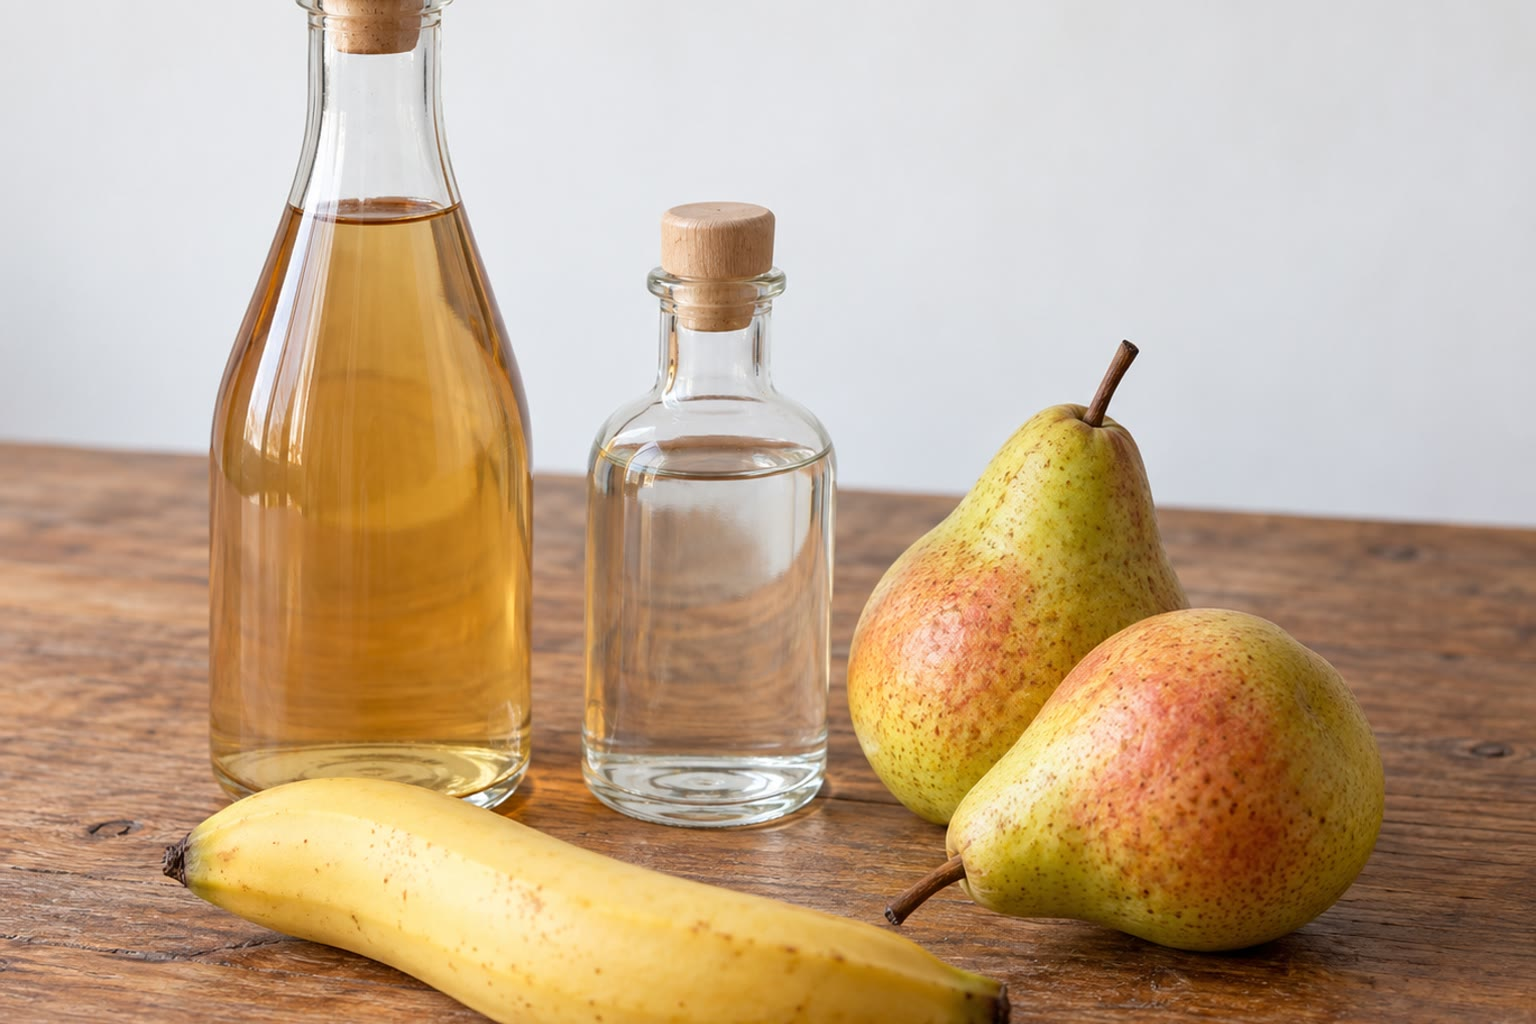
\includegraphics[width=0.5\linewidth]{images/book1/ai/g11-still-life-esters.jpg}

{\small Vinegar, a \omterm{def:g6:solutions-and-solubility:solute}{solvent}, fruit: each smell comes from a different
group of \omterm{def:g7:atoms-and-molecules:atom}{atoms} on a carbon skeleton.}
\end{omfigure}

\section{Functional groups}

\begin{definition}[Functional group]\label{def:g11:functional-groups:functional-group}
A \emph{functional group}\index{functional group} is a group of \omterm{def:g7:atoms-and-molecules:atom}{atoms},
other than the carbon and hydrogen \omterm{def:g7:atoms-and-molecules:atom}{atoms} of the skeleton linked only by
single bonds, that gives a \omterm{def:g7:atoms-and-molecules:molecule}{molecule} its characteristic reactions. The
compounds that share a functional \omterm{def:g9:periodic-table-first-look:period}{group} form a family.
\end{definition}

\begin{omfigure}
\renewcommand{\arraystretch}{1.35}
\footnotesize
\begin{tabular}{@{}l@{\enspace}l@{\enspace}l@{\enspace}l@{\enspace}l@{}}
\hline
group & formula & family & name ending & example \\
\hline
hydroxyl & \ce{-OH} & \omterm{def:g11:functional-groups:alcohol}{alcohol} & \emph{-ol} & ethanol, \ce{CH3-CH2-OH} \\
carbonyl (end) & \ce{-CHO} & \omterm{def:g11:functional-groups:carbonyl}{aldehyde} & \emph{-al} & ethanal, \ce{CH3-CHO} \\
carbonyl (inside) & \ce{C-CO-C} & \omterm{def:g11:functional-groups:carbonyl}{ketone} & \emph{-one} & propanone, \ce{CH3-CO-CH3} \\
carboxyl & \ce{-COOH} & \omterm{def:g11:functional-groups:carboxylic-acid}{carboxylic acid} & \emph{-oic acid} & ethanoic acid, \ce{CH3-COOH} \\
\omterm{def:g11:functional-groups:carboxylic-acid}{ester} & \ce{C-COO-C} & \omterm{def:g11:functional-groups:carboxylic-acid}{ester} & \emph{-yl \ldots-oate} & ethyl ethanoate, \ce{CH3-COO-CH2-CH3} \\
\omterm{def:g11:functional-groups:amine}{amine} & \ce{-NH2} & \omterm{def:g11:functional-groups:amine}{amine} & \emph{-amine} & ethanamine, \ce{CH3-CH2-NH2} \\
\omterm{def:g11:functional-groups:amine}{amide} & \ce{-CONH2} & \omterm{def:g11:functional-groups:amine}{amide} & \emph{-amide} & ethanamide, \ce{CH3-CONH2} \\
\omterm{def:g10:electron-shells:family}{halogen} & \ce{C-X} & \omterm{def:g11:functional-groups:halogenoalkane}{halogenoalkane} & prefix \emph{chloro-}, \ldots & chloromethane, \ce{CH3Cl} \\
\omterm{def:g10:lewis-and-shape:multiple-bond}{double bond} & \ce{C=C} & \omterm{def:g11:functional-groups:halogenoalkane}{alkene} & \emph{-ene} & ethene, \ce{CH2=CH2} \\
\hline
\end{tabular}\par\medskip

\setchemfig{atom sep=1.4em}
\begin{tabular}{@{}c@{\quad}c@{\quad}c@{\quad}c@{\quad}c@{}}
\chemfig{R-C(=[2]O)-H} & \chemfig{R-C(=[2]O)-R'} & \chemfig{R-C(=[2]O)-O-H} &
\chemfig{R-C(=[2]O)-O-R'} & \chemfig{R-C(=[2]O)-N(-[1]H)-[7]H} \\
\small \omterm{def:g11:functional-groups:carbonyl}{aldehyde} & \small \omterm{def:g11:functional-groups:carbonyl}{ketone} & \small \omterm{def:g11:functional-groups:carboxylic-acid}{carboxylic acid} & \small \omterm{def:g11:functional-groups:carboxylic-acid}{ester} &
\small \omterm{def:g11:functional-groups:amine}{amide}
\end{tabular}\par\medskip

{\small The main \omterm{def:g11:functional-groups:functional-group}{functional groups}, and the five built on a carbonyl
group \ce{C=O}, drawn in full. R and R$'$ stand for carbon chains (alkyl
groups) and X for a \omterm{def:g10:electron-shells:family}{halogen} \omterm{def:g7:atoms-and-molecules:atom}{atom} (F, Cl, Br, I).}
\end{omfigure}

\section{Alcohols and their class}

\begin{definition}[Alcohol, class of an alcohol]\label{def:g11:functional-groups:alcohol}
An \emph{alcohol}\index{alcohol} has a hydroxyl group \ce{-OH} bonded to
a carbon \omterm{def:g7:atoms-and-molecules:atom}{atom} that has only single bonds. The \emph{class of an
alcohol}\index{class of an alcohol} is primary, secondary or tertiary
according to whether the carbon \omterm{def:g7:atoms-and-molecules:atom}{atom} bearing the \ce{-OH} is bonded to
one, two or three other carbon \omterm{def:g7:atoms-and-molecules:atom}{atoms}. (Methanol, \ce{CH3OH}, whose
carbon is bonded to none, is counted with the primary alcohols.)
\end{definition}

\begin{omfigure}
\setchemfig{atom sep=1.9em}
\begin{tabular}{ccc}
\chemfig{-[:30]-[:-30]-[:30]-[:-30]OH} &
\chemfig{-[:30](-[:90]OH)-[:-30]-[:30]} &
\chemfig{-[:0](-[:90]OH)(-[:-90])-[:0]} \\[4pt]
\small butan-1-ol & \small butan-2-ol & \small 2-methylpropan-2-ol \\
\small \textbf{primary} & \small \textbf{secondary} & \small \textbf{tertiary} \\
\small (C of \ce{-OH}: 1 carbon neighbour) & \small (2 neighbours) &
\small (3 neighbours)
\end{tabular}

{\small Three \omterm{def:g11:organic-skeletons:isomer}{isomers} \ce{C4H10O}, three classes of \omterm{def:g11:functional-groups:alcohol}{alcohol}.}
\end{omfigure}

\section{Aldehydes, ketones, acids and esters}

\begin{definition}[Aldehyde, ketone]\label{def:g11:functional-groups:carbonyl}
A carbonyl group is a \ce{C=O} \omterm{def:g10:lewis-and-shape:multiple-bond}{double bond}. If its carbon \omterm{def:g7:atoms-and-molecules:atom}{atom} is at the
end of the chain (bonded to at least one hydrogen \omterm{def:g7:atoms-and-molecules:atom}{atom}), the compound is
an \emph{aldehyde}\index{aldehyde}; if it is inside the chain (bonded to
two carbon \omterm{def:g7:atoms-and-molecules:atom}{atoms}), the compound is a \emph{ketone}\index{ketone}.
\end{definition}

\begin{definition}[Carboxylic acid, ester]\label{def:g11:functional-groups:carboxylic-acid}
A \emph{carboxylic acid}\index{carboxylic acid} has a carboxyl group
\ce{-COOH}, a carbonyl and a hydroxyl on the same carbon \omterm{def:g7:atoms-and-molecules:atom}{atom}. An
\emph{ester}\index{ester} has the group \ce{-COO-} between two carbon
chains: it is related to an acid, whose \ce{-OH} has been replaced by an
\ce{-O-}R$'$ coming from an \omterm{def:g11:functional-groups:alcohol}{alcohol}.
\end{definition}

\begin{example}[Ethyl ethanoate]\label{ex:g11:functional-groups:ethyl-ethanoate}
The \omterm{def:g6:solutions-and-solubility:solute}{solvent} ethyl ethanoate, \ce{CH3-COO-CH2-CH3}, smells of pear drops
and nail-varnish remover. Its ``acid part'', \ce{CH3-CO}, comes from
ethanoic acid \ce{CH3-COOH} and gives the second word of the name,
\emph{ethanoate}; its ``\omterm{def:g11:functional-groups:alcohol}{alcohol} part'', \ce{O-CH2-CH3}, comes from
ethanol \ce{CH3-CH2-OH} and gives the first word, \emph{ethyl}. A
later chapter shows how an \omterm{def:g11:functional-groups:carboxylic-acid}{ester} is made from its acid and its \omterm{def:g11:functional-groups:alcohol}{alcohol}.
\end{example}

\begin{omfigure}
\setchemfig{atom sep=2.2em}
\chemfig{@{a}H_3C-@{c}C(=[2]@{o}O)-@{x}O-CH_2-@{z}CH_3}
\chemmove{
  \fill[omProp, opacity=0.14, rounded corners]
    ($(a.south west)+(-0.12,-0.15)$) rectangle ($(o.north east)+(0.25,0.12)$);
  \fill[omDef, opacity=0.14, rounded corners]
    ($(x.south west)+(-0.2,-0.15)$) rectangle ($(z.north east)+(0.4,0.75)$);
  \node[omProp, anchor=north east, align=right, font=\small] at ($(c.south)+(0.15,-0.25)$)
    {acid part, from ethanoic acid:\\ \emph{ethanoate}};
  \node[omDef, anchor=north west, align=left, font=\small] at ($(x.south)+(0.05,-0.25)$)
    {alcohol part, from ethanol:\\ \emph{ethyl}};}
\par\vspace{1.4cm}

{\small Naming an \omterm{def:g11:functional-groups:carboxylic-acid}{ester}: the \omterm{def:g11:functional-groups:alcohol}{alcohol} part gives an alkyl name
(\emph{ethyl}), the acid part an ending in \emph{-oate}
(\emph{ethanoate}); the name is ``ethyl ethanoate''.}
\end{omfigure}

\section{Amines, amides, halogenoalkanes and alkenes}


\begin{definition}[Amine, amide]\label{def:g11:functional-groups:amine}
An \emph{amine}\index{amine} has a nitrogen \omterm{def:g7:atoms-and-molecules:atom}{atom} bonded to a carbon chain
by a single bond, as in \ce{-NH2}. An \emph{amide}\index{amide} has a nitrogen \omterm{def:g7:atoms-and-molecules:atom}{atom}
bonded to the carbon of a carbonyl group, as in \ce{-CO-NH2}.
\end{definition}

\begin{definition}[Halogenoalkane, alkene]\label{def:g11:functional-groups:halogenoalkane}
A \emph{halogenoalkane}\index{halogenoalkane} is an \omterm{def:g11:organic-skeletons:alkane}{alkane} in which one
or more hydrogen \omterm{def:g7:atoms-and-molecules:atom}{atoms} are replaced by \omterm{def:g10:electron-shells:family}{halogen} \omterm{def:g7:atoms-and-molecules:atom}{atoms} (F, Cl, Br, I). An
\emph{alkene}\index{alkene} has a carbon--carbon \omterm{def:g10:lewis-and-shape:multiple-bond}{double bond}, \ce{C=C}.
\end{definition}

\begin{remark}[Smells and groups]\label{rem:g11:functional-groups:smells}
Many small \omterm{def:g11:functional-groups:amine}{amines} smell of rotten fish, and the smell of fish that is no
longer fresh is largely due to them. Many small \omterm{def:g11:functional-groups:carboxylic-acid}{esters} smell of fruit.
Small \omterm{def:g11:functional-groups:carboxylic-acid}{carboxylic acids} smell sharp, like vinegar; propanone, a \omterm{def:g11:functional-groups:carbonyl}{ketone},
is the familiar \omterm{def:g6:solutions-and-solubility:solute}{solvent} smell of nail-varnish remover.
\end{remark}

\section{Naming}

\begin{method}[Naming an organic compound with one functional group]\label{met:g11:functional-groups:naming}
\begin{enumerate}
  \item Find the longest carbon chain that \emph{contains} the carbon of
        the \omterm{def:g11:functional-groups:functional-group}{functional group} (or, for an \omterm{def:g11:functional-groups:alcohol}{alcohol} or an \omterm{def:g11:functional-groups:amine}{amine}, the carbon
        that bears it): it gives the root.
  \item Number the chain from the end that gives the \omterm{def:g11:functional-groups:functional-group}{functional group} the
        lowest number.
  \item Replace the \emph{-e} of the \omterm{def:g11:organic-skeletons:alkane}{alkane} by the ending of the family,
        preceded by the position of the group if needed: propan-2-ol,
        butan-2-one. (\omterm{def:g11:functional-groups:carbonyl}{Aldehydes}, acids and \omterm{def:g11:functional-groups:amine}{amides} have their group at
        carbon 1: no number.)
  \item Add the alkyl substituents as prefixes, with their positions,
        as for \omterm{def:g11:organic-skeletons:alkane}{alkanes}; a \omterm{def:g10:electron-shells:family}{halogen} is always a prefix (2-chloropropane).
\end{enumerate}
\end{method}

\begin{example}[Four names]\label{ex:g11:functional-groups:names}
\setchemfig{atom sep=1.7em}
\chemfig{-[:30](-[:90]OH)-[:-30]} is propan-2-ol (a secondary \omterm{def:g11:functional-groups:alcohol}{alcohol});
\chemfig{-[:30](=[:90]O)-[:-30]-[:30]} is butan-2-one;
\chemfig{-[:30]-[:-30]-[:30](=[:90]O)-[:-30]OH} is butanoic acid;
\chemfig{-[:30](-[:90])-[:-30]-[:30]=[:-30]O} is 3-methylbutanal.
\end{example}

\begin{omfigure}
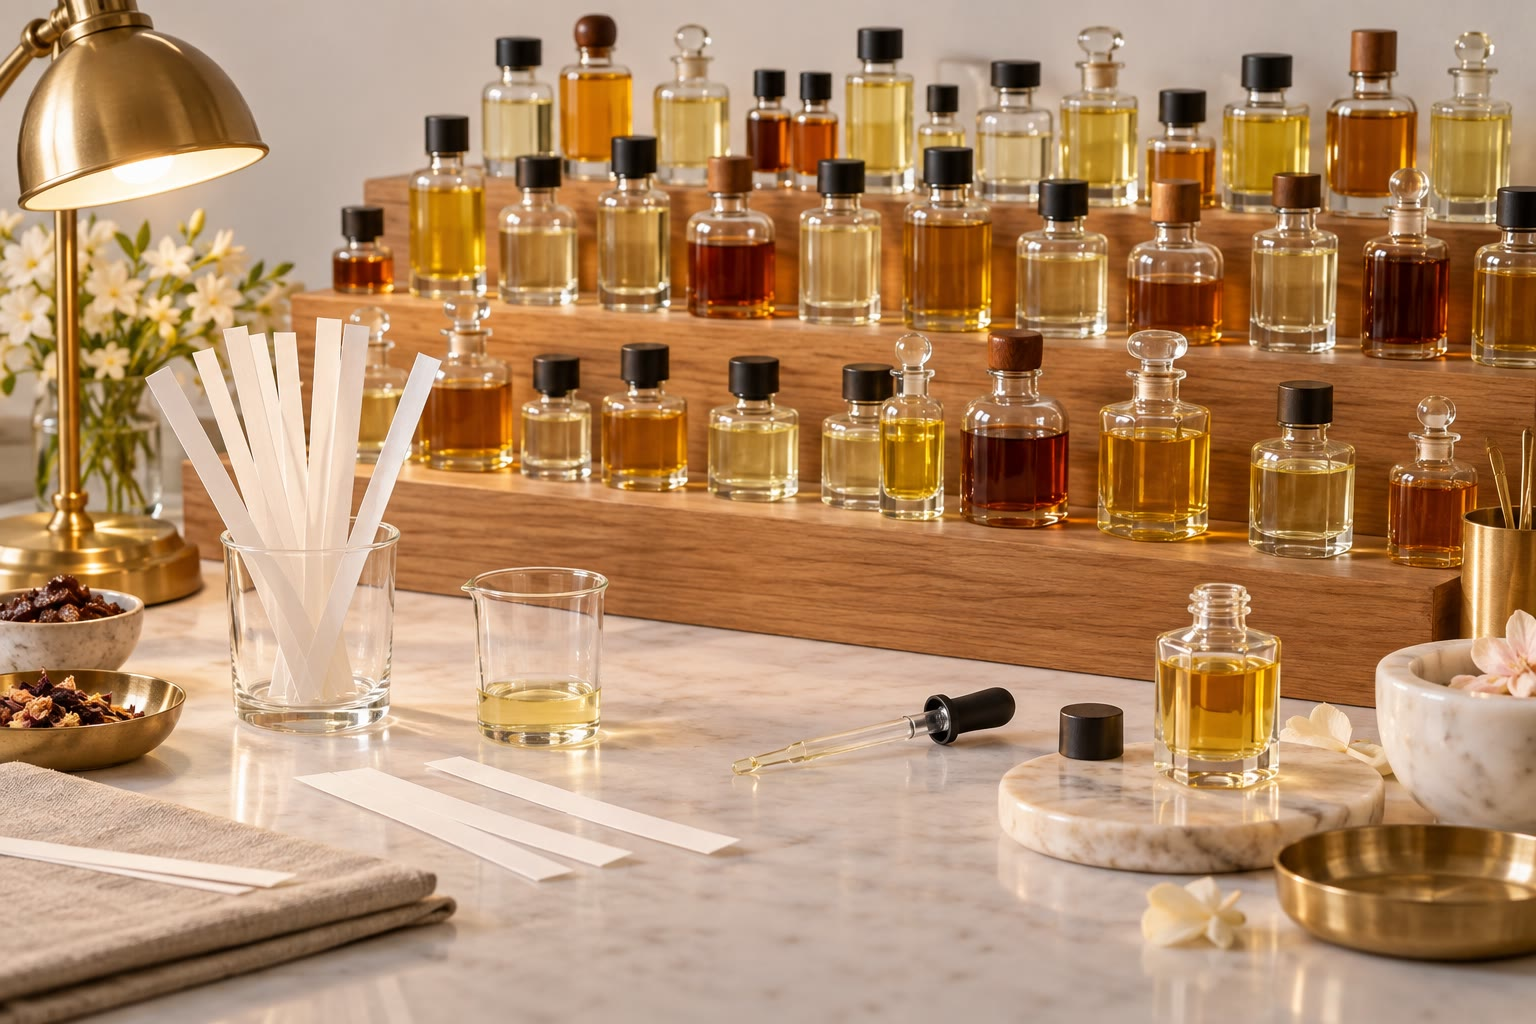
\includegraphics[width=0.48\linewidth]{images/book1/ai/g11-perfumer-lab.jpg}

{\small A perfumer's bench: many of the bottles hold \omterm{def:g11:functional-groups:carboxylic-acid}{esters}, \omterm{def:g11:functional-groups:alcohol}{alcohols},
\omterm{def:g11:functional-groups:carbonyl}{aldehydes} and \omterm{def:g11:functional-groups:carbonyl}{ketones}.}
\end{omfigure}

\begin{safety}{\ghs[0.82cm]{GHS02}\ghs[0.82cm]{GHS05}\ghs[0.82cm]{GHS07}}
% ledger: ghs:acetone, ghs:acetic-acid
Propanone is highly flammable and irritating to the eyes; its vapour
makes one drowsy. Pure ethanoic acid is flammable and causes severe
burns of the skin and the eyes; vinegar is a dilute solution of it.
Smells are never tested by sniffing a flask: the vapour is wafted
gently towards the nose with the hand, and only when the teacher says
so.
\end{safety}

\section{Exercises}


\begin{exercise}[$\star$]\label{exo:g11:functional-groups:1}
Name the \omterm{def:g11:functional-groups:functional-group}{functional group} and the family of each compound:
\ce{CH3-CH2-CH2-OH}; \ce{CH3-CO-CH2-CH3}; \ce{CH3-CH2-COOH};
\ce{CH3-COO-CH3}; \ce{CH3-CH2-NH2}.
\end{exercise}

\begin{exercise}[$\star$]\label{exo:g11:functional-groups:2}
Name: \ce{CH3-OH}; \ce{CH3-CH2-CH2-OH}; \ce{HCOOH}; \ce{CH3-CH2-CHO};
\ce{CH3-CO-CH3}.
\end{exercise}

\begin{exercise}[$\star$]\label{exo:g11:functional-groups:3}
To which family does each compound belong: butan-2-ol, pentanal, methyl
propanoate, propanamide, 2-bromopropane, but-1-ene?
\end{exercise}

\begin{exercise}[$\star$]\label{exo:g11:functional-groups:4}
Write the \omterm{def:g11:organic-skeletons:formulas}{semi-structural formulas} of propanal and of propanone. Which
is the \omterm{def:g11:functional-groups:carbonyl}{aldehyde}? How do you tell?
\end{exercise}

\begin{exercise}[$\star$]\label{exo:g11:functional-groups:5}
Give the class of propan-1-ol, propan-2-ol and 2-methylpropan-2-ol.
\end{exercise}

\begin{exercise}[$\star\star$]\label{exo:g11:functional-groups:6}
Draw the \omterm{def:g11:organic-skeletons:formulas}{skeletal formulas} of pentan-3-ol, 2-methylbutanoic acid,
hexan-2-one and propyl ethanoate.
\end{exercise}

\begin{exercise}[$\star\star$]\label{exo:g11:functional-groups:7}
Propanal and propanone have the same \omterm{def:g11:organic-skeletons:formulas}{molecular formula}. Give it. Are
they \omterm{def:g11:organic-skeletons:isomer}{isomers}? Do they have the same \omterm{def:g11:functional-groups:functional-group}{functional group}?
\end{exercise}

\begin{exercise}[$\star\star$]\label{exo:g11:functional-groups:8}
Write the \omterm{def:g11:organic-skeletons:formulas}{semi-structural formula} and the name of the \omterm{def:g11:functional-groups:carboxylic-acid}{ester} whose acid
part comes from methanoic acid \ce{HCOOH} and whose \omterm{def:g11:functional-groups:alcohol}{alcohol} part comes
from ethanol; then of the \omterm{def:g11:functional-groups:carboxylic-acid}{ester} from ethanoic acid and propan-1-ol.
\end{exercise}

\begin{exercise}[$\star\star$]\label{exo:g11:functional-groups:9}
Name the \omterm{def:g11:functional-groups:carboxylic-acid}{esters} \ce{CH3-COO-CH3}, \ce{CH3-CH2-COO-CH2-CH3} and
\ce{HCOO-CH3}, and give the acid and the \omterm{def:g11:functional-groups:alcohol}{alcohol} each is related to.
\end{exercise}

\begin{exercise}[$\star\star$]\label{exo:g11:functional-groups:10}
Draw and name the four \omterm{def:g11:functional-groups:alcohol}{alcohols} of formula \ce{C4H10O}, and give the
class of each.
\end{exercise}

\begin{exercise}[$\star\star$]\label{exo:g11:functional-groups:11}
Using the table of groups: what is the family of \ce{CH3-CO-NH2}? What
ending does the name of an \omterm{def:g11:functional-groups:halogenoalkane}{alkene} take? Which two families have a
carbonyl group with an oxygen or nitrogen \omterm{def:g7:atoms-and-molecules:atom}{atom} on the same carbon?
\end{exercise}

\begin{exercise}[$\star\star\star$]\label{exo:g11:functional-groups:12}
Circle and name the \omterm{def:g11:functional-groups:functional-group}{functional groups} of aspirin and of paracetamol.
(An \ce{-OH} bonded directly to a ring like that of paracetamol is called
a phenol group; it behaves differently from an \omterm{def:g11:functional-groups:alcohol}{alcohol}.)
\begin{center}
\setchemfig{atom sep=1.6em}
\chemfig{*6(-=-(-COOH)=(-O-[:150]C(=[:90]O)-[:210]H_3C)-=)}
\qquad
\chemfig{*6((-OH)=-=(-N(-[2]H)-[7]C(=[6]O)-[1]CH_3)-=-)}
\\[2pt] \small aspirin \hspace{4.2cm} paracetamol
\end{center}
\end{exercise}

\begin{exercise}[$\star\star\star$]\label{exo:g11:functional-groups:13}
% ledger: bp:C2H5OH, bp:CH3OCH3
Ethanol \ce{CH3-CH2-OH} and methoxymethane \ce{CH3-O-CH3} have the same
\omterm{def:g11:organic-skeletons:formulas}{molecular formula}. Give it. Methoxymethane belongs to a family not in
the table, the ethers. Which of the two can form \omterm{def:g11:polarity-and-cohesion:hydrogen-bond}{hydrogen bonds} between
its own \omterm{def:g7:atoms-and-molecules:molecule}{molecules}? Which boils higher (one boils at \qty{78}{\celsius},
the other at \qty{-25}{\celsius})?
\end{exercise}

\begin{exercise}[$\star\star\star$]\label{exo:g11:functional-groups:14}
Lactic acid, made by tired muscles, is
\chemfig{CH_3-CH(-[2]OH)-COOH}. Name its two \omterm{def:g11:functional-groups:functional-group}{functional groups}. When a
\omterm{def:g7:atoms-and-molecules:molecule}{molecule} has an acid group and another group, the acid gives the ending
and the other group becomes a prefix (\emph{hydroxy-} for \ce{-OH},
\emph{amino-} for \ce{-NH2}). Name lactic acid, then glycine,
\ce{H2N-CH2-COOH}.
\end{exercise}

\begin{exercise}[$\star\star\star$]\label{exo:g11:functional-groups:15}
Wine left open to the \omterm{def:g4:air-a-mixture-of-gases:air}{air} turns into vinegar: ethanol becomes ethanoic
acid, through ethanal. Write the semi-structural and \omterm{def:g11:organic-skeletons:formulas}{molecular formulas}
of the three compounds and their families. What changes in the formula
at each step?
\end{exercise}

\section{Problem: Fruit Flavours}

\begin{problem}[{Weekend problem --- a flavour chemist builds the smell of
banana: what is the molar mass of the key molecule?}]
\label{pb:g11:functional-groups:1}
% ledger: aw:C, aw:H, aw:O
A flavour chemist has five compounds on her bench:
\begin{center}
\begin{tabular}{ll}
A & \chemfig{CH_3-C(=[2]O)-O-CH_2-CH_2-CH(-[2]CH_3)-CH_3} \\[16pt]
B & \chemfig{HO-CH_2-CH_2-CH(-[2]CH_3)-CH_3} \\[10pt]
C & \ce{CH3-COOH} \\
D & \ce{CH3-CH2-CH2-CH2-CH2-CHO} \\
E & \ce{CH3-CH2-CH2-COO-CH2-CH3}
\end{tabular}
\end{center}
A smells of banana and pear drops, B of malt, C of vinegar, D of cut
grass, E of pineapple.

\medskip
\noindent\textbf{Part I --- Groups and families.}
\begin{enumerate}
  \item Name the \omterm{def:g11:functional-groups:functional-group}{functional group} of each compound.
  \item Give the family of each.
  \item Which compounds are \omterm{def:g11:functional-groups:carboxylic-acid}{esters}? Which smells do they have?
  \item What is the class of the \omterm{def:g11:functional-groups:alcohol}{alcohol} B?
  \item Give the \omterm{def:g11:organic-skeletons:formulas}{molecular formula} of D, and draw an isomer of D that is
        a \omterm{def:g11:functional-groups:carbonyl}{ketone}.
\end{enumerate}

\medskip
\noindent\textbf{Part II --- Names.}
\begin{enumerate}[resume]
  \item Name B (find the longest chain that holds the carbon bearing
        \ce{-OH}).
  \item Name C and D.
  \item Name E, and give the acid and the \omterm{def:g11:functional-groups:alcohol}{alcohol} it is related to.
  \item Explain the name of A, 3-methylbutyl ethanoate: which part comes
        from the acid, which from the \omterm{def:g11:functional-groups:alcohol}{alcohol}?
\end{enumerate}

\medskip
\noindent\textbf{Part III --- From an acid and an \omterm{def:g11:functional-groups:alcohol}{alcohol}.}
\begin{enumerate}[resume]
  \item To which two compounds of the bench is A related?
  \item Give the \omterm{def:g11:organic-skeletons:formulas}{molecular formulas} of A, B and C.
  \item An \omterm{def:g11:functional-groups:carboxylic-acid}{ester} is made from its acid and its \omterm{def:g11:functional-groups:alcohol}{alcohol} with loss of one
        small \omterm{def:g7:atoms-and-molecules:molecule}{molecule}. Using the formulas, find which.
  \item Write the equation of the formation of A, in \omterm{def:g11:organic-skeletons:formulas}{molecular formulas},
        and check that it is balanced.
\end{enumerate}

\medskip
\noindent\textbf{Part IV --- Molar masses.}
\begin{enumerate}[resume]
  \item Compute the molar masses of B and C.
  \item Deduce the \omterm{def:g10:the-mole:molar-mass}{molar mass} of A from the equation of question 13.
  \item Compute the \omterm{def:g10:the-mole:molar-mass}{molar mass} of A directly from its formula, and
        compare.
  \item An unknown fruity sample is found to have a \omterm{def:g10:the-mole:molar-mass}{molar mass} close to
        \qty{116}{g/mol}. Is it A or E?
  \item Heptanoic acid, \ce{CH3-(CH2)5-COOH}, smells rancid. Show that it
        is an isomer of A. Can a \omterm{def:g10:the-mole:molar-mass}{molar mass} alone identify a compound?
  \item Why do chemists say the smell belongs to the \omterm{def:g11:functional-groups:functional-group}{functional group} as
        much as to the skeleton? Use A and heptanoic acid.
  \item State the final answer: what is the \omterm{def:g10:the-mole:molar-mass}{molar mass} of the banana
        \omterm{def:g11:functional-groups:carboxylic-acid}{ester}, 3-methylbutyl ethanoate?
\end{enumerate}
\end{problem}
